% Options for packages loaded elsewhere
\PassOptionsToPackage{unicode}{hyperref}
\PassOptionsToPackage{hyphens}{url}
%
\documentclass[
  12pt,
]{article}
\usepackage{amsmath,amssymb}
\usepackage{lmodern}
\usepackage{iftex}
\ifPDFTeX
  \usepackage[T1]{fontenc}
  \usepackage[utf8]{inputenc}
  \usepackage{textcomp} % provide euro and other symbols
\else % if luatex or xetex
  \usepackage{unicode-math}
  \defaultfontfeatures{Scale=MatchLowercase}
  \defaultfontfeatures[\rmfamily]{Ligatures=TeX,Scale=1}
  \setmainfont[]{Times New Roman}
\fi
% Use upquote if available, for straight quotes in verbatim environments
\IfFileExists{upquote.sty}{\usepackage{upquote}}{}
\IfFileExists{microtype.sty}{% use microtype if available
  \usepackage[]{microtype}
  \UseMicrotypeSet[protrusion]{basicmath} % disable protrusion for tt fonts
}{}
\makeatletter
\@ifundefined{KOMAClassName}{% if non-KOMA class
  \IfFileExists{parskip.sty}{%
    \usepackage{parskip}
  }{% else
    \setlength{\parindent}{0pt}
    \setlength{\parskip}{6pt plus 2pt minus 1pt}}
}{% if KOMA class
  \KOMAoptions{parskip=half}}
\makeatother
\usepackage{xcolor}
\IfFileExists{xurl.sty}{\usepackage{xurl}}{} % add URL line breaks if available
\IfFileExists{bookmark.sty}{\usepackage{bookmark}}{\usepackage{hyperref}}
\hypersetup{
  pdftitle={Insert title of project here},
  pdfauthor={Name},
  hidelinks,
  pdfcreator={LaTeX via pandoc}}
\urlstyle{same} % disable monospaced font for URLs
\usepackage[margin=2.54cm]{geometry}
\usepackage{color}
\usepackage{fancyvrb}
\newcommand{\VerbBar}{|}
\newcommand{\VERB}{\Verb[commandchars=\\\{\}]}
\DefineVerbatimEnvironment{Highlighting}{Verbatim}{commandchars=\\\{\}}
% Add ',fontsize=\small' for more characters per line
\usepackage{framed}
\definecolor{shadecolor}{RGB}{248,248,248}
\newenvironment{Shaded}{\begin{snugshade}}{\end{snugshade}}
\newcommand{\AlertTok}[1]{\textcolor[rgb]{0.94,0.16,0.16}{#1}}
\newcommand{\AnnotationTok}[1]{\textcolor[rgb]{0.56,0.35,0.01}{\textbf{\textit{#1}}}}
\newcommand{\AttributeTok}[1]{\textcolor[rgb]{0.77,0.63,0.00}{#1}}
\newcommand{\BaseNTok}[1]{\textcolor[rgb]{0.00,0.00,0.81}{#1}}
\newcommand{\BuiltInTok}[1]{#1}
\newcommand{\CharTok}[1]{\textcolor[rgb]{0.31,0.60,0.02}{#1}}
\newcommand{\CommentTok}[1]{\textcolor[rgb]{0.56,0.35,0.01}{\textit{#1}}}
\newcommand{\CommentVarTok}[1]{\textcolor[rgb]{0.56,0.35,0.01}{\textbf{\textit{#1}}}}
\newcommand{\ConstantTok}[1]{\textcolor[rgb]{0.00,0.00,0.00}{#1}}
\newcommand{\ControlFlowTok}[1]{\textcolor[rgb]{0.13,0.29,0.53}{\textbf{#1}}}
\newcommand{\DataTypeTok}[1]{\textcolor[rgb]{0.13,0.29,0.53}{#1}}
\newcommand{\DecValTok}[1]{\textcolor[rgb]{0.00,0.00,0.81}{#1}}
\newcommand{\DocumentationTok}[1]{\textcolor[rgb]{0.56,0.35,0.01}{\textbf{\textit{#1}}}}
\newcommand{\ErrorTok}[1]{\textcolor[rgb]{0.64,0.00,0.00}{\textbf{#1}}}
\newcommand{\ExtensionTok}[1]{#1}
\newcommand{\FloatTok}[1]{\textcolor[rgb]{0.00,0.00,0.81}{#1}}
\newcommand{\FunctionTok}[1]{\textcolor[rgb]{0.00,0.00,0.00}{#1}}
\newcommand{\ImportTok}[1]{#1}
\newcommand{\InformationTok}[1]{\textcolor[rgb]{0.56,0.35,0.01}{\textbf{\textit{#1}}}}
\newcommand{\KeywordTok}[1]{\textcolor[rgb]{0.13,0.29,0.53}{\textbf{#1}}}
\newcommand{\NormalTok}[1]{#1}
\newcommand{\OperatorTok}[1]{\textcolor[rgb]{0.81,0.36,0.00}{\textbf{#1}}}
\newcommand{\OtherTok}[1]{\textcolor[rgb]{0.56,0.35,0.01}{#1}}
\newcommand{\PreprocessorTok}[1]{\textcolor[rgb]{0.56,0.35,0.01}{\textit{#1}}}
\newcommand{\RegionMarkerTok}[1]{#1}
\newcommand{\SpecialCharTok}[1]{\textcolor[rgb]{0.00,0.00,0.00}{#1}}
\newcommand{\SpecialStringTok}[1]{\textcolor[rgb]{0.31,0.60,0.02}{#1}}
\newcommand{\StringTok}[1]{\textcolor[rgb]{0.31,0.60,0.02}{#1}}
\newcommand{\VariableTok}[1]{\textcolor[rgb]{0.00,0.00,0.00}{#1}}
\newcommand{\VerbatimStringTok}[1]{\textcolor[rgb]{0.31,0.60,0.02}{#1}}
\newcommand{\WarningTok}[1]{\textcolor[rgb]{0.56,0.35,0.01}{\textbf{\textit{#1}}}}
\usepackage{graphicx}
\makeatletter
\def\maxwidth{\ifdim\Gin@nat@width>\linewidth\linewidth\else\Gin@nat@width\fi}
\def\maxheight{\ifdim\Gin@nat@height>\textheight\textheight\else\Gin@nat@height\fi}
\makeatother
% Scale images if necessary, so that they will not overflow the page
% margins by default, and it is still possible to overwrite the defaults
% using explicit options in \includegraphics[width, height, ...]{}
\setkeys{Gin}{width=\maxwidth,height=\maxheight,keepaspectratio}
% Set default figure placement to htbp
\makeatletter
\def\fps@figure{htbp}
\makeatother
\setlength{\emergencystretch}{3em} % prevent overfull lines
\providecommand{\tightlist}{%
  \setlength{\itemsep}{0pt}\setlength{\parskip}{0pt}}
\setcounter{secnumdepth}{5}
\ifLuaTeX
  \usepackage{selnolig}  % disable illegal ligatures
\fi

\title{Insert title of project here}
\usepackage{etoolbox}
\makeatletter
\providecommand{\subtitle}[1]{% add subtitle to \maketitle
  \apptocmd{\@title}{\par {\large #1 \par}}{}{}
}
\makeatother
\subtitle{Web address for GitHub repository}
\author{Name}
\date{}

\begin{document}
\maketitle

\newpage
\tableofcontents

\newpage
\listoftables

\newpage
\listoffigures

\newpage

\hypertarget{rationale-and-research-questions}{%
\section{Rationale and Research
Questions}\label{rationale-and-research-questions}}

\#We perform analysis based on the following sub-questions. \#How is
groundwater table related to precipitation? \#How is groundwater table
level related to local river discharge? \#How is ground water table
level related to local withdraws?

\newpage

\hypertarget{dataset-information}{%
\section{Dataset Information}\label{dataset-information}}

\newpage

\hypertarget{exploratory-analysis}{%
\section{Exploratory Analysis}\label{exploratory-analysis}}

\begin{Shaded}
\begin{Highlighting}[]
\CommentTok{\#Regular Water Resources}
\NormalTok{CapeFearRiverDischarge }\OtherTok{\textless{}{-}} \FunctionTok{readNWISdv}\NormalTok{(}\AttributeTok{siteNumbers =} \StringTok{"02096500"}\NormalTok{,}
                                  \AttributeTok{parameterCd =} \StringTok{"00060"}\NormalTok{, }\CommentTok{\# discharge (ft3/s)}
                                  \AttributeTok{startDate =} \StringTok{"1990{-}01{-}01"}\NormalTok{,}
                                  \AttributeTok{endDate =} \StringTok{"2021{-}12{-}31"}\NormalTok{)}
\FunctionTok{names}\NormalTok{(CapeFearRiverDischarge)[}\DecValTok{4}\SpecialCharTok{:}\DecValTok{5}\NormalTok{] }\OtherTok{\textless{}{-}} \FunctionTok{c}\NormalTok{(}\StringTok{"Discharge"}\NormalTok{, }\StringTok{"Approval.Code"}\NormalTok{)}
\FunctionTok{c}\NormalTok{(}\FunctionTok{min}\NormalTok{(CapeFearRiverDischarge}\SpecialCharTok{$}\NormalTok{Date), }\FunctionTok{max}\NormalTok{(CapeFearRiverDischarge}\SpecialCharTok{$}\NormalTok{Date))}
\end{Highlighting}
\end{Shaded}

\begin{verbatim}
## [1] "1990-01-01" "2021-12-31"
\end{verbatim}

\begin{Shaded}
\begin{Highlighting}[]
\CommentTok{\#"1990{-}01{-}01" "2021{-}12{-}31"}
\NormalTok{CapeFearRiverDischarge\_Monthly }\OtherTok{\textless{}{-}}\NormalTok{ CapeFearRiverDischarge }\SpecialCharTok{\%\textgreater{}\%}
  \FunctionTok{mutate}\NormalTok{(}\AttributeTok{Month =} \FunctionTok{format}\NormalTok{(Date,}\StringTok{"\%Y{-}\%m"}\NormalTok{)) }\SpecialCharTok{\%\textgreater{}\%}
  \FunctionTok{group\_by}\NormalTok{(Month) }\SpecialCharTok{\%\textgreater{}\%}
  \FunctionTok{summarise}\NormalTok{(}\AttributeTok{Mean\_Discharge\_Bymonth =} \FunctionTok{mean}\NormalTok{(Discharge),}
            \AttributeTok{River =} \FunctionTok{paste}\NormalTok{(}\StringTok{"Cape Fear River"}\NormalTok{))}

\NormalTok{FlatRiverDischarge }\OtherTok{\textless{}{-}} \FunctionTok{readNWISdv}\NormalTok{(}\AttributeTok{siteNumbers =} \StringTok{"02085500"}\NormalTok{,}
                                  \AttributeTok{parameterCd =} \StringTok{"00060"}\NormalTok{, }\CommentTok{\# discharge (ft3/s)}
                                  \AttributeTok{startDate =} \StringTok{"1990{-}01{-}01"}\NormalTok{,}
                                  \AttributeTok{endDate =} \StringTok{"2021{-}12{-}31"}\NormalTok{)}
\FunctionTok{names}\NormalTok{(FlatRiverDischarge)[}\DecValTok{4}\SpecialCharTok{:}\DecValTok{5}\NormalTok{] }\OtherTok{\textless{}{-}} \FunctionTok{c}\NormalTok{(}\StringTok{"Discharge"}\NormalTok{, }\StringTok{"Approval.Code"}\NormalTok{)}
\FunctionTok{c}\NormalTok{(}\FunctionTok{min}\NormalTok{(FlatRiverDischarge}\SpecialCharTok{$}\NormalTok{Date), }\FunctionTok{max}\NormalTok{(FlatRiverDischarge}\SpecialCharTok{$}\NormalTok{Date))}
\end{Highlighting}
\end{Shaded}

\begin{verbatim}
## [1] "1990-01-01" "2021-12-31"
\end{verbatim}

\begin{Shaded}
\begin{Highlighting}[]
\CommentTok{\#"1990{-}01{-}01" "2021{-}12{-}31"}
\NormalTok{FlatRiverDischarge\_Monthly }\OtherTok{\textless{}{-}}\NormalTok{ FlatRiverDischarge }\SpecialCharTok{\%\textgreater{}\%}
  \FunctionTok{mutate}\NormalTok{(}\AttributeTok{Month =} \FunctionTok{format}\NormalTok{(Date,}\StringTok{"\%Y{-}\%m"}\NormalTok{)) }\SpecialCharTok{\%\textgreater{}\%}
  \FunctionTok{group\_by}\NormalTok{(Month) }\SpecialCharTok{\%\textgreater{}\%}
  \FunctionTok{summarise}\NormalTok{(}\AttributeTok{Mean\_Discharge\_Bymonth =} \FunctionTok{mean}\NormalTok{(Discharge),}
            \AttributeTok{River =} \FunctionTok{paste}\NormalTok{(}\StringTok{"Flat River"}\NormalTok{))}

\NormalTok{LittleRiverDischarge }\OtherTok{\textless{}{-}} \FunctionTok{readNWISdv}\NormalTok{(}\AttributeTok{siteNumbers =} \StringTok{"0208524975"}\NormalTok{,}
                                  \AttributeTok{parameterCd =} \StringTok{"00060"}\NormalTok{, }\CommentTok{\# discharge (ft3/s)}
                                  \AttributeTok{startDate =} \StringTok{"1990{-}01{-}01"}\NormalTok{,}
                                  \AttributeTok{endDate =} \StringTok{"2021{-}12{-}31"}\NormalTok{)}
\FunctionTok{names}\NormalTok{(LittleRiverDischarge)[}\DecValTok{4}\SpecialCharTok{:}\DecValTok{5}\NormalTok{] }\OtherTok{\textless{}{-}} \FunctionTok{c}\NormalTok{(}\StringTok{"Discharge"}\NormalTok{, }\StringTok{"Approval.Code"}\NormalTok{)}
\FunctionTok{c}\NormalTok{(}\FunctionTok{min}\NormalTok{(LittleRiverDischarge}\SpecialCharTok{$}\NormalTok{Date), }\FunctionTok{max}\NormalTok{(LittleRiverDischarge}\SpecialCharTok{$}\NormalTok{Date))}
\end{Highlighting}
\end{Shaded}

\begin{verbatim}
## [1] "1995-10-24" "2021-12-31"
\end{verbatim}

\begin{Shaded}
\begin{Highlighting}[]
\CommentTok{\#"1995{-}10{-}24" "2021{-}12{-}31"}
\NormalTok{LittleRiverDischarge\_Monthly }\OtherTok{\textless{}{-}}\NormalTok{ LittleRiverDischarge }\SpecialCharTok{\%\textgreater{}\%}
  \FunctionTok{mutate}\NormalTok{(}\AttributeTok{Month =} \FunctionTok{format}\NormalTok{(Date,}\StringTok{"\%Y{-}\%m"}\NormalTok{)) }\SpecialCharTok{\%\textgreater{}\%}
  \FunctionTok{group\_by}\NormalTok{(Month) }\SpecialCharTok{\%\textgreater{}\%}
  \FunctionTok{summarise}\NormalTok{(}\AttributeTok{Mean\_Discharge\_Bymonth =} \FunctionTok{mean}\NormalTok{(Discharge),}
            \AttributeTok{River =} \FunctionTok{paste}\NormalTok{(}\StringTok{"Little River"}\NormalTok{))}

\CommentTok{\#Emergency Water Resources}
\NormalTok{EnoRiverDischarge }\OtherTok{\textless{}{-}} \FunctionTok{readNWISdv}\NormalTok{(}\AttributeTok{siteNumbers =} \StringTok{"02085070"}\NormalTok{,}
                                  \AttributeTok{parameterCd =} \StringTok{"00060"}\NormalTok{, }\CommentTok{\# discharge (ft3/s)}
                                  \AttributeTok{startDate =} \StringTok{"1990{-}01{-}01"}\NormalTok{,}
                                  \AttributeTok{endDate =} \StringTok{"2021{-}12{-}31"}\NormalTok{)}
\FunctionTok{names}\NormalTok{(EnoRiverDischarge)[}\DecValTok{4}\SpecialCharTok{:}\DecValTok{5}\NormalTok{] }\OtherTok{\textless{}{-}} \FunctionTok{c}\NormalTok{(}\StringTok{"Discharge"}\NormalTok{, }\StringTok{"Approval.Code"}\NormalTok{)}
\FunctionTok{c}\NormalTok{(}\FunctionTok{min}\NormalTok{(EnoRiverDischarge}\SpecialCharTok{$}\NormalTok{Date), }\FunctionTok{max}\NormalTok{(EnoRiverDischarge}\SpecialCharTok{$}\NormalTok{Date))}
\end{Highlighting}
\end{Shaded}

\begin{verbatim}
## [1] "1990-01-01" "2021-12-31"
\end{verbatim}

\begin{Shaded}
\begin{Highlighting}[]
\CommentTok{\#"1990{-}01{-}01" "2021{-}12{-}31"}
\NormalTok{EnoRiverDischarge\_Monthly }\OtherTok{\textless{}{-}}\NormalTok{ EnoRiverDischarge }\SpecialCharTok{\%\textgreater{}\%}
  \FunctionTok{mutate}\NormalTok{(}\AttributeTok{Month =} \FunctionTok{format}\NormalTok{(Date,}\StringTok{"\%Y{-}\%m"}\NormalTok{)) }\SpecialCharTok{\%\textgreater{}\%}
  \FunctionTok{group\_by}\NormalTok{(Month) }\SpecialCharTok{\%\textgreater{}\%}
  \FunctionTok{summarise}\NormalTok{(}\AttributeTok{Mean\_Discharge\_Bymonth =} \FunctionTok{mean}\NormalTok{(Discharge),}
            \AttributeTok{River =} \FunctionTok{paste}\NormalTok{(}\StringTok{"Eno River"}\NormalTok{))}

\CommentTok{\#Surrounding Water Resources (Unused)}
\NormalTok{EllerbeCreekDischarge }\OtherTok{\textless{}{-}} \FunctionTok{readNWISdv}\NormalTok{(}\AttributeTok{siteNumbers =} \StringTok{"0208675010"}\NormalTok{,}
                                  \AttributeTok{parameterCd =} \StringTok{"00060"}\NormalTok{, }\CommentTok{\# discharge (ft3/s)}
                                  \AttributeTok{startDate =} \StringTok{"1990{-}01{-}01"}\NormalTok{,}
                                  \AttributeTok{endDate =} \StringTok{"2021{-}12{-}31"}\NormalTok{)}
\FunctionTok{names}\NormalTok{(EllerbeCreekDischarge)[}\DecValTok{4}\SpecialCharTok{:}\DecValTok{5}\NormalTok{] }\OtherTok{\textless{}{-}} \FunctionTok{c}\NormalTok{(}\StringTok{"Discharge"}\NormalTok{, }\StringTok{"Approval.Code"}\NormalTok{)}
\FunctionTok{c}\NormalTok{(}\FunctionTok{min}\NormalTok{(EllerbeCreekDischarge}\SpecialCharTok{$}\NormalTok{Date), }\FunctionTok{max}\NormalTok{(EllerbeCreekDischarge}\SpecialCharTok{$}\NormalTok{Date))}
\end{Highlighting}
\end{Shaded}

\begin{verbatim}
## [1] "2008-08-01" "2021-12-31"
\end{verbatim}

\begin{Shaded}
\begin{Highlighting}[]
\CommentTok{\#"2008{-}08{-}01" "2021{-}12{-}31"}
\NormalTok{EllerbeCreekDischarge\_Monthly }\OtherTok{\textless{}{-}}\NormalTok{ EllerbeCreekDischarge }\SpecialCharTok{\%\textgreater{}\%}
  \FunctionTok{mutate}\NormalTok{(}\AttributeTok{Month =} \FunctionTok{format}\NormalTok{(Date,}\StringTok{"\%Y{-}\%m"}\NormalTok{)) }\SpecialCharTok{\%\textgreater{}\%}
  \FunctionTok{group\_by}\NormalTok{(Month) }\SpecialCharTok{\%\textgreater{}\%}
  \FunctionTok{summarise}\NormalTok{(}\AttributeTok{Mean\_Discharge\_Bymonth =} \FunctionTok{mean}\NormalTok{(Discharge),}
            \AttributeTok{River =} \FunctionTok{paste}\NormalTok{(}\StringTok{"Ellerbe Creek"}\NormalTok{))}

\NormalTok{SandyCreekDischarge }\OtherTok{\textless{}{-}} \FunctionTok{readNWISdv}\NormalTok{(}\AttributeTok{siteNumbers =} \StringTok{"0209722970"}\NormalTok{,}
                                  \AttributeTok{parameterCd =} \StringTok{"00060"}\NormalTok{, }\CommentTok{\# discharge (ft3/s)}
                                  \AttributeTok{startDate =} \StringTok{"1990{-}01{-}01"}\NormalTok{,}
                                  \AttributeTok{endDate =} \StringTok{"2021{-}12{-}31"}\NormalTok{)}
\FunctionTok{names}\NormalTok{(SandyCreekDischarge)[}\DecValTok{4}\SpecialCharTok{:}\DecValTok{5}\NormalTok{] }\OtherTok{\textless{}{-}} \FunctionTok{c}\NormalTok{(}\StringTok{"Discharge"}\NormalTok{, }\StringTok{"Approval.Code"}\NormalTok{)}
\FunctionTok{c}\NormalTok{(}\FunctionTok{min}\NormalTok{(SandyCreekDischarge}\SpecialCharTok{$}\NormalTok{Date), }\FunctionTok{max}\NormalTok{(SandyCreekDischarge}\SpecialCharTok{$}\NormalTok{Date))}
\end{Highlighting}
\end{Shaded}

\begin{verbatim}
## [1] "2008-08-01" "2021-12-31"
\end{verbatim}

\begin{Shaded}
\begin{Highlighting}[]
\CommentTok{\#"2008{-}08{-}01" "2021{-}12{-}31"}
\NormalTok{SandyCreekDischarge\_Monthly }\OtherTok{\textless{}{-}}\NormalTok{ SandyCreekDischarge }\SpecialCharTok{\%\textgreater{}\%}
  \FunctionTok{mutate}\NormalTok{(}\AttributeTok{Month =} \FunctionTok{format}\NormalTok{(Date,}\StringTok{"\%Y{-}\%m"}\NormalTok{)) }\SpecialCharTok{\%\textgreater{}\%}
  \FunctionTok{group\_by}\NormalTok{(Month) }\SpecialCharTok{\%\textgreater{}\%}
  \FunctionTok{summarise}\NormalTok{(}\AttributeTok{Mean\_Discharge\_Bymonth =} \FunctionTok{mean}\NormalTok{(Discharge),}
            \AttributeTok{River =} \FunctionTok{paste}\NormalTok{(}\StringTok{"Sandy Creek"}\NormalTok{))}

\NormalTok{ThirdForkCreekDischarge }\OtherTok{\textless{}{-}} \FunctionTok{readNWISdv}\NormalTok{(}\AttributeTok{siteNumbers =} \StringTok{"0209725960"}\NormalTok{,}
                                  \AttributeTok{parameterCd =} \StringTok{"00060"}\NormalTok{, }\CommentTok{\# discharge (ft3/s)}
                                  \AttributeTok{startDate =} \StringTok{"1990{-}01{-}01"}\NormalTok{,}
                                  \AttributeTok{endDate =} \StringTok{"2021{-}12{-}31"}\NormalTok{)}
\FunctionTok{names}\NormalTok{(ThirdForkCreekDischarge)[}\DecValTok{4}\SpecialCharTok{:}\DecValTok{5}\NormalTok{] }\OtherTok{\textless{}{-}} \FunctionTok{c}\NormalTok{(}\StringTok{"Discharge"}\NormalTok{, }\StringTok{"Approval.Code"}\NormalTok{)}
\FunctionTok{c}\NormalTok{(}\FunctionTok{min}\NormalTok{(ThirdForkCreekDischarge}\SpecialCharTok{$}\NormalTok{Date), }\FunctionTok{max}\NormalTok{(ThirdForkCreekDischarge}\SpecialCharTok{$}\NormalTok{Date))}
\end{Highlighting}
\end{Shaded}

\begin{verbatim}
## [1] "2017-06-16" "2021-12-31"
\end{verbatim}

\begin{Shaded}
\begin{Highlighting}[]
\CommentTok{\#"2017{-}06{-}16" "2021{-}12{-}31"}
\NormalTok{ThirdForkCreekDischarge\_Monthly }\OtherTok{\textless{}{-}}\NormalTok{ ThirdForkCreekDischarge }\SpecialCharTok{\%\textgreater{}\%}
  \FunctionTok{mutate}\NormalTok{(}\AttributeTok{Month =} \FunctionTok{format}\NormalTok{(Date,}\StringTok{"\%Y{-}\%m"}\NormalTok{)) }\SpecialCharTok{\%\textgreater{}\%}
  \FunctionTok{group\_by}\NormalTok{(Month) }\SpecialCharTok{\%\textgreater{}\%}
  \FunctionTok{summarise}\NormalTok{(}\AttributeTok{Mean\_Discharge\_Bymonth =} \FunctionTok{mean}\NormalTok{(Discharge),}
            \AttributeTok{River =} \FunctionTok{paste}\NormalTok{(}\StringTok{"Third Fork Creek"}\NormalTok{))}
\end{Highlighting}
\end{Shaded}

\begin{Shaded}
\begin{Highlighting}[]
\NormalTok{GroundParams }\OtherTok{\textless{}{-}} \FunctionTok{whatNWISdata}\NormalTok{(}\AttributeTok{siteNumbers =} \StringTok{"355944079013401"}\NormalTok{)}
\NormalTok{DurhamGroundwater }\OtherTok{\textless{}{-}} \FunctionTok{readNWISdv}\NormalTok{(}\AttributeTok{siteNumbers =} \StringTok{"355944079013401"}\NormalTok{,}
                                 \AttributeTok{parameterCd =} \StringTok{"72019"}\NormalTok{, }\CommentTok{\# /62610/Groundwater level above NGVD 1929 (feet)}
                                 \AttributeTok{statCd =} \StringTok{"00002"}\NormalTok{,}
                                 \AttributeTok{startDate =} \StringTok{"2014{-}01{-}01"}\NormalTok{,}
                                 \AttributeTok{endDate =} \StringTok{"2021{-}12{-}31"}\NormalTok{)}
\FunctionTok{names}\NormalTok{(DurhamGroundwater)[}\DecValTok{4}\SpecialCharTok{:}\DecValTok{5}\NormalTok{] }\OtherTok{\textless{}{-}} \FunctionTok{c}\NormalTok{(}\StringTok{"Groundwater\_Table\_feet"}\NormalTok{, }\StringTok{"Approval.Code"}\NormalTok{)}
\FunctionTok{c}\NormalTok{(}\FunctionTok{min}\NormalTok{(DurhamGroundwater}\SpecialCharTok{$}\NormalTok{Date), }\FunctionTok{max}\NormalTok{(DurhamGroundwater}\SpecialCharTok{$}\NormalTok{Date))}
\end{Highlighting}
\end{Shaded}

\begin{verbatim}
## [1] "2014-01-01" "2021-12-31"
\end{verbatim}

\begin{Shaded}
\begin{Highlighting}[]
\CommentTok{\# }
\end{Highlighting}
\end{Shaded}

\begin{Shaded}
\begin{Highlighting}[]
\CommentTok{\#the PSWID of Durham}
\NormalTok{durham\_pswid }\OtherTok{=} \StringTok{\textquotesingle{}03{-}32{-}010\textquotesingle{}}
\CommentTok{\#years with records}
\NormalTok{the\_years }\OtherTok{=} \FunctionTok{c}\NormalTok{(}\DecValTok{2018}\SpecialCharTok{:}\DecValTok{2021}\NormalTok{)}

\CommentTok{\#Scrap Function}
\NormalTok{scrape.totalwithdrawal }\OtherTok{\textless{}{-}} \ControlFlowTok{function}\NormalTok{(the\_pswid, the\_year)\{}
\NormalTok{  the\_website }\OtherTok{\textless{}{-}} \FunctionTok{read\_html}\NormalTok{(}\FunctionTok{paste0}\NormalTok{(}\StringTok{\textquotesingle{}https://www.ncwater.org/WUDC/app/LWSP/report.php?pwsid=\textquotesingle{}}\NormalTok{, }
\NormalTok{                                  the\_pswid, }\StringTok{\textquotesingle{}\&year=\textquotesingle{}}\NormalTok{, the\_year))}
  
\NormalTok{  water\_system\_name\_tag }\OtherTok{\textless{}{-}} \StringTok{\textquotesingle{}div+ table tr:nth{-}child(1) td:nth{-}child(2)\textquotesingle{}}
\NormalTok{  ownership\_tag }\OtherTok{\textless{}{-}} \StringTok{\textquotesingle{}div+ table tr:nth{-}child(2) td:nth{-}child(4)\textquotesingle{}}
\NormalTok{  avg\_daily\_use\_tag }\OtherTok{\textless{}{-}} \StringTok{\textquotesingle{}.fancy{-}table:nth{-}child(31) th+ td\textquotesingle{}}
  
\NormalTok{  water\_system\_name }\OtherTok{\textless{}{-}}\NormalTok{ the\_website }\SpecialCharTok{\%\textgreater{}\%} \FunctionTok{html\_nodes}\NormalTok{(water\_system\_name\_tag) }\SpecialCharTok{\%\textgreater{}\%} \FunctionTok{html\_text}\NormalTok{()}
\NormalTok{  ownership }\OtherTok{\textless{}{-}}\NormalTok{ the\_website }\SpecialCharTok{\%\textgreater{}\%}   \FunctionTok{html\_nodes}\NormalTok{(ownership\_tag) }\SpecialCharTok{\%\textgreater{}\%}  \FunctionTok{html\_text}\NormalTok{()}
\NormalTok{  avg\_daily\_use }\OtherTok{\textless{}{-}}\NormalTok{ the\_website }\SpecialCharTok{\%\textgreater{}\%} \FunctionTok{html\_nodes}\NormalTok{(avg\_daily\_use\_tag) }\SpecialCharTok{\%\textgreater{}\%} \FunctionTok{html\_text}\NormalTok{()}
  
\NormalTok{  df\_withdrawals }\OtherTok{\textless{}{-}} \FunctionTok{data.frame}\NormalTok{(}\StringTok{"Year"} \OtherTok{=} \FunctionTok{rep}\NormalTok{(the\_year,}\DecValTok{12}\NormalTok{),}
                               \StringTok{"Month"} \OtherTok{=} \FunctionTok{rep}\NormalTok{(}\DecValTok{1}\SpecialCharTok{:}\DecValTok{12}\NormalTok{),}
                               \StringTok{"Avg\_Daily\_Use\_mgd"} \OtherTok{=} \FunctionTok{as.numeric}\NormalTok{(avg\_daily\_use)) }\SpecialCharTok{\%\textgreater{}\%} 
    \FunctionTok{mutate}\NormalTok{(}\AttributeTok{Water\_System\_name =} \SpecialCharTok{!!}\NormalTok{water\_system\_name,}
         \AttributeTok{Ownership =} \SpecialCharTok{!!}\NormalTok{ownership,}
         \AttributeTok{Date =} \FunctionTok{my}\NormalTok{(}\FunctionTok{paste}\NormalTok{(Month,}\StringTok{"{-}"}\NormalTok{,Year)))}
  
  \FunctionTok{print}\NormalTok{(}\FunctionTok{paste}\NormalTok{(}\StringTok{\textquotesingle{}The Pswid =\textquotesingle{}}\NormalTok{, the\_pswid, }\StringTok{\textquotesingle{}, The Year =\textquotesingle{}}\NormalTok{, the\_year))}
  \FunctionTok{return}\NormalTok{(df\_withdrawals)}
\NormalTok{\}}

\NormalTok{total\_withdrawal }\OtherTok{\textless{}{-}} \FunctionTok{map}\NormalTok{(the\_years, scrape.totalwithdrawal, }\AttributeTok{the\_pswid =}\NormalTok{ durham\_pswid)}
\end{Highlighting}
\end{Shaded}

\begin{verbatim}
## [1] "The Pswid = 03-32-010 , The Year = 2018"
## [1] "The Pswid = 03-32-010 , The Year = 2019"
## [1] "The Pswid = 03-32-010 , The Year = 2020"
## [1] "The Pswid = 03-32-010 , The Year = 2021"
\end{verbatim}

\begin{Shaded}
\begin{Highlighting}[]
\NormalTok{total\_withdrawal }\OtherTok{\textless{}{-}} \FunctionTok{bind\_rows}\NormalTok{(total\_withdrawal)}
\end{Highlighting}
\end{Shaded}

\begin{Shaded}
\begin{Highlighting}[]
\CommentTok{\#the PSWID of Durham}
\NormalTok{durham\_pswid }\OtherTok{=} \StringTok{\textquotesingle{}03{-}32{-}010\textquotesingle{}}
\CommentTok{\#years with records}
\NormalTok{the\_years }\OtherTok{=} \FunctionTok{c}\NormalTok{(}\DecValTok{2018}\SpecialCharTok{:}\DecValTok{2021}\NormalTok{)}

\NormalTok{scrape.withdrawal.distribution }\OtherTok{\textless{}{-}} \ControlFlowTok{function}\NormalTok{(the\_pswid, the\_year)\{}
\NormalTok{  the\_website }\OtherTok{\textless{}{-}} \FunctionTok{read\_html}\NormalTok{(}\FunctionTok{paste0}\NormalTok{(}\StringTok{\textquotesingle{}https://www.ncwater.org/WUDC/app/LWSP/report.php?pwsid=\textquotesingle{}}\NormalTok{, }
\NormalTok{                                  the\_pswid, }\StringTok{\textquotesingle{}\&year=\textquotesingle{}}\NormalTok{, the\_year))}
  
\NormalTok{  water\_system\_name\_tag }\OtherTok{\textless{}{-}} \StringTok{\textquotesingle{}div+ table tr:nth{-}child(1) td:nth{-}child(2)\textquotesingle{}}
\NormalTok{  ownership\_tag }\OtherTok{\textless{}{-}} \StringTok{\textquotesingle{}div+ table tr:nth{-}child(2) td:nth{-}child(4)\textquotesingle{}}
\NormalTok{  stream\_name\_tag }\OtherTok{\textless{}{-}} \StringTok{\textquotesingle{}.fancy{-}table:nth{-}child(35) .left:nth{-}child(1)\textquotesingle{}}
\NormalTok{  avg\_daily\_use\_tag }\OtherTok{\textless{}{-}} \StringTok{\textquotesingle{}.fancy{-}table:nth{-}child(35) .left\textasciitilde{} .left+ td\textquotesingle{}}
\NormalTok{  the\_numberofdaysused\_tag }\OtherTok{\textless{}{-}} \StringTok{\textquotesingle{}.fancy{-}table:nth{-}child(35) td:nth{-}child(4)\textquotesingle{}}
  
\NormalTok{  water\_system\_name }\OtherTok{\textless{}{-}}\NormalTok{ the\_website }\SpecialCharTok{\%\textgreater{}\%} \FunctionTok{html\_nodes}\NormalTok{(water\_system\_name\_tag) }\SpecialCharTok{\%\textgreater{}\%} \FunctionTok{html\_text}\NormalTok{()}
\NormalTok{  ownership }\OtherTok{\textless{}{-}}\NormalTok{ the\_website }\SpecialCharTok{\%\textgreater{}\%}   \FunctionTok{html\_nodes}\NormalTok{(ownership\_tag) }\SpecialCharTok{\%\textgreater{}\%}  \FunctionTok{html\_text}\NormalTok{()}
\NormalTok{  stream\_name }\OtherTok{\textless{}{-}}\NormalTok{ the\_website }\SpecialCharTok{\%\textgreater{}\%} \FunctionTok{html\_nodes}\NormalTok{(stream\_name\_tag) }\SpecialCharTok{\%\textgreater{}\%} \FunctionTok{html\_text}\NormalTok{()}
\NormalTok{  avg\_daily\_use }\OtherTok{\textless{}{-}}\NormalTok{ the\_website }\SpecialCharTok{\%\textgreater{}\%} \FunctionTok{html\_nodes}\NormalTok{(avg\_daily\_use\_tag) }\SpecialCharTok{\%\textgreater{}\%} \FunctionTok{html\_text}\NormalTok{()}
\NormalTok{  the\_numberofdaysused }\OtherTok{\textless{}{-}}\NormalTok{ the\_website }\SpecialCharTok{\%\textgreater{}\%} \FunctionTok{html\_nodes}\NormalTok{(the\_numberofdaysused\_tag) }\SpecialCharTok{\%\textgreater{}\%} \FunctionTok{html\_text}\NormalTok{()}
  
\NormalTok{  df\_withdrawals }\OtherTok{\textless{}{-}} \FunctionTok{data.frame}\NormalTok{(}\StringTok{"Year"} \OtherTok{=} \FunctionTok{rep}\NormalTok{(the\_year,}\DecValTok{5}\NormalTok{),}
                               \StringTok{"Stream\_Name"} \OtherTok{=}\NormalTok{ stream\_name,}
                               \StringTok{"Avg\_Daily\_Use\_mgd"} \OtherTok{=} \FunctionTok{as.numeric}\NormalTok{(avg\_daily\_use),}
                               \StringTok{"Number\_of\_Days\_Used"} \OtherTok{=} \FunctionTok{as.numeric}\NormalTok{(the\_numberofdaysused)) }\SpecialCharTok{\%\textgreater{}\%} 
    \FunctionTok{mutate}\NormalTok{(}\AttributeTok{Water\_System\_name =} \SpecialCharTok{!!}\NormalTok{water\_system\_name,}
         \AttributeTok{Ownership =} \SpecialCharTok{!!}\NormalTok{ownership)}
  
  \FunctionTok{print}\NormalTok{(}\FunctionTok{paste}\NormalTok{(}\StringTok{\textquotesingle{}The Pswid =\textquotesingle{}}\NormalTok{, the\_pswid, }\StringTok{\textquotesingle{}, The Year =\textquotesingle{}}\NormalTok{, the\_year))}
  \FunctionTok{return}\NormalTok{(df\_withdrawals)}
\NormalTok{\}}

\NormalTok{withdrawal\_distribution }\OtherTok{\textless{}{-}} \FunctionTok{map}\NormalTok{(the\_years, scrape.withdrawal.distribution, }\AttributeTok{the\_pswid =}\NormalTok{ durham\_pswid)}
\end{Highlighting}
\end{Shaded}

\begin{verbatim}
## [1] "The Pswid = 03-32-010 , The Year = 2018"
## [1] "The Pswid = 03-32-010 , The Year = 2019"
## [1] "The Pswid = 03-32-010 , The Year = 2020"
## [1] "The Pswid = 03-32-010 , The Year = 2021"
\end{verbatim}

\begin{Shaded}
\begin{Highlighting}[]
\NormalTok{withdrawal\_distribution }\OtherTok{\textless{}{-}} \FunctionTok{bind\_rows}\NormalTok{(withdrawal\_distribution)}
\end{Highlighting}
\end{Shaded}

\begin{Shaded}
\begin{Highlighting}[]
\CommentTok{\#Water{-}use industries\textquotesingle{} sites }
\CommentTok{\#https://www.ncwater.org/WUDC/app/WWATR/report}
\NormalTok{Brentwood }\OtherTok{\textless{}{-}} \StringTok{"0218{-}0068"}
\NormalTok{CanterburyEstates }\OtherTok{\textless{}{-}} \StringTok{"0218{-}0086"}
\NormalTok{CardensCreek }\OtherTok{\textless{}{-}} \StringTok{"0218{-}0088"}
\NormalTok{FoxRun }\OtherTok{\textless{}{-}} \StringTok{"0218{-}0199"}
\NormalTok{Greymoss }\OtherTok{\textless{}{-}} \StringTok{"0218{-}0229"}
\NormalTok{Hardscrabble }\OtherTok{\textless{}{-}} \StringTok{"0218{-}0238"}
\NormalTok{LakeRidge }\OtherTok{\textless{}{-}} \StringTok{"0218{-}0313"}
\NormalTok{Masonwoods }\OtherTok{\textless{}{-}} \StringTok{"0218{-}0349"}
\NormalTok{RedMountain }\OtherTok{\textless{}{-}} \StringTok{"0218{-}0460"}
\NormalTok{TrappersCreek }\OtherTok{\textless{}{-}} \StringTok{"0218{-}0608"}
\NormalTok{Tyndrum }\OtherTok{\textless{}{-}} \StringTok{"0218{-}0619"}
\NormalTok{Wexford }\OtherTok{\textless{}{-}} \StringTok{"0218{-}0646"}
\NormalTok{WillowHill }\OtherTok{\textless{}{-}} \StringTok{"0218{-}0658"}
\NormalTok{HeatherGlen }\OtherTok{\textless{}{-}} \StringTok{"0378{-}0038"}
\NormalTok{ColvardFarms }\OtherTok{\textless{}{-}} \StringTok{"0427{-}0001"}
\NormalTok{CroasdaileCountryClub }\OtherTok{\textless{}{-}} \StringTok{"0419{-}0001"}
\NormalTok{RougemontQuarry }\OtherTok{\textless{}{-}} \StringTok{"0340{-}0003"}
\NormalTok{Durham.sites }\OtherTok{\textless{}{-}} \FunctionTok{c}\NormalTok{(Brentwood, CanterburyEstates, CardensCreek, FoxRun, Greymoss, Hardscrabble, LakeRidge, Masonwoods, RedMountain, TrappersCreek, Tyndrum, Wexford, WillowHill, HeatherGlen, ColvardFarms, CroasdaileCountryClub, RougemontQuarry)}

\CommentTok{\#years with records}
\NormalTok{the\_years }\OtherTok{=} \FunctionTok{c}\NormalTok{(}\DecValTok{2007}\SpecialCharTok{:}\DecValTok{2021}\NormalTok{)}

\CommentTok{\#Scraping Function}
\NormalTok{scrape.industrywithdrawals }\OtherTok{\textless{}{-}} \ControlFlowTok{function}\NormalTok{(the\_year, the\_facility)\{}
  \CommentTok{\#Retrieve the website contents }
\NormalTok{  the\_website }\OtherTok{\textless{}{-}} \FunctionTok{read\_html}\NormalTok{(}\FunctionTok{paste0}\NormalTok{(}\StringTok{\textquotesingle{}https://www.ncwater.org/WUDC/app/WWATR/report/view/\textquotesingle{}}\NormalTok{, }
\NormalTok{                                  the\_facility, }\StringTok{\textquotesingle{}/\textquotesingle{}}\NormalTok{, the\_year))}
  
  \CommentTok{\#Set the element address variables (determined in the previous step)}
\NormalTok{  the\_registrant\_tag }\OtherTok{\textless{}{-}} \StringTok{\textquotesingle{}.table tr:nth{-}child(1) td:nth{-}child(2)\textquotesingle{}}
\NormalTok{  the\_facility\_name\_tag }\OtherTok{\textless{}{-}} \StringTok{\textquotesingle{}tr:nth{-}child(2) th+ .left:nth{-}child(2)\textquotesingle{}}
\NormalTok{  the\_facility\_id\_tag }\OtherTok{\textless{}{-}} \StringTok{\textquotesingle{}tr:nth{-}child(2) .left\textasciitilde{} .left+ td.left\textquotesingle{}}
\NormalTok{  the\_data\_tag }\OtherTok{\textless{}{-}} \StringTok{\textquotesingle{}.table:nth{-}child(7) td:nth{-}child(7) , .table:nth{-}child(7) td:nth{-}child(3)\textquotesingle{}}
\NormalTok{  the\_numberofdaysused\_tag }\OtherTok{\textless{}{-}} \StringTok{\textquotesingle{}.table:nth{-}child(7) th+ td\textquotesingle{}}
  
  \CommentTok{\#Scrape the data items}
\NormalTok{  the\_registrant }\OtherTok{\textless{}{-}}\NormalTok{ the\_website }\SpecialCharTok{\%\textgreater{}\%} \FunctionTok{html\_nodes}\NormalTok{(the\_registrant\_tag) }\SpecialCharTok{\%\textgreater{}\%} \FunctionTok{html\_text}\NormalTok{()}
\NormalTok{  the\_facility\_name }\OtherTok{\textless{}{-}}\NormalTok{ the\_website }\SpecialCharTok{\%\textgreater{}\%}   \FunctionTok{html\_nodes}\NormalTok{(the\_facility\_name\_tag) }\SpecialCharTok{\%\textgreater{}\%}  \FunctionTok{html\_text}\NormalTok{()}
\NormalTok{  the\_facility\_type }\OtherTok{\textless{}{-}}\NormalTok{ the\_website }\SpecialCharTok{\%\textgreater{}\%} \FunctionTok{html\_nodes}\NormalTok{(the\_facility\_id\_tag) }\SpecialCharTok{\%\textgreater{}\%} \FunctionTok{html\_text}\NormalTok{()}
\NormalTok{  avg\_withdrawals }\OtherTok{\textless{}{-}}\NormalTok{ the\_website }\SpecialCharTok{\%\textgreater{}\%} \FunctionTok{html\_nodes}\NormalTok{(the\_data\_tag) }\SpecialCharTok{\%\textgreater{}\%} \FunctionTok{html\_text}\NormalTok{()}
\NormalTok{  the\_numberofdaysused }\OtherTok{\textless{}{-}}\NormalTok{ the\_website }\SpecialCharTok{\%\textgreater{}\%} \FunctionTok{html\_nodes}\NormalTok{(the\_numberofdaysused\_tag) }\SpecialCharTok{\%\textgreater{}\%} \FunctionTok{html\_text}\NormalTok{()}
  
  \CommentTok{\#Convert to a dataframe}
\NormalTok{  df\_withdrawals }\OtherTok{\textless{}{-}} \FunctionTok{data.frame}\NormalTok{(}\StringTok{"Year"} \OtherTok{=} \FunctionTok{rep}\NormalTok{(the\_year,}\DecValTok{12}\NormalTok{),}
                               \StringTok{"Month"} \OtherTok{=} \FunctionTok{rep}\NormalTok{(}\DecValTok{1}\SpecialCharTok{:}\DecValTok{12}\NormalTok{),}
                               \StringTok{"Avg\_Withdrawals\_mgd"} \OtherTok{=} \FunctionTok{as.numeric}\NormalTok{(avg\_withdrawals),}
                               \StringTok{"Number\_of\_Days\_Used"} \OtherTok{=} \FunctionTok{as.numeric}\NormalTok{(the\_numberofdaysused)) }\SpecialCharTok{\%\textgreater{}\%} 
    \FunctionTok{mutate}\NormalTok{(}\AttributeTok{Registrant =} \SpecialCharTok{!!}\NormalTok{the\_registrant,}
           \AttributeTok{Facility\_name =} \SpecialCharTok{!!}\NormalTok{the\_facility\_name,}
           \AttributeTok{Facility\_type =} \SpecialCharTok{!!}\NormalTok{the\_facility\_type,}
           \AttributeTok{Date =} \FunctionTok{my}\NormalTok{(}\FunctionTok{paste}\NormalTok{(Month,}\StringTok{"{-}"}\NormalTok{,Year)))}
  
  \CommentTok{\#Pause for a moment {-} scraping etiquette}
  \CommentTok{\#Sys.sleep(1) \#uncomment this if you are doing bulk scraping!}
  
  \CommentTok{\#Return the dataframe}
  \FunctionTok{return}\NormalTok{(df\_withdrawals)}
\NormalTok{\}}

\NormalTok{industry\_withdrawal }\OtherTok{\textless{}{-}} \FunctionTok{cross2}\NormalTok{(the\_years, Durham.sites) }\SpecialCharTok{\%\textgreater{}\%} 
  \FunctionTok{map}\NormalTok{(}\FunctionTok{lift}\NormalTok{(scrape.industrywithdrawals)) }\SpecialCharTok{\%\textgreater{}\%} 
  \FunctionTok{bind\_rows}\NormalTok{()}

\NormalTok{industry\_withdrawal\_Monthly }\OtherTok{\textless{}{-}}\NormalTok{ industry\_withdrawal }\SpecialCharTok{\%\textgreater{}\%}
  \FunctionTok{select}\NormalTok{(Date, Avg\_Withdrawals\_mgd) }\SpecialCharTok{\%\textgreater{}\%}
  \FunctionTok{mutate}\NormalTok{(}\AttributeTok{Month =} \FunctionTok{format}\NormalTok{(Date,}\StringTok{"\%Y{-}\%m"}\NormalTok{)) }\SpecialCharTok{\%\textgreater{}\%}
  \FunctionTok{group\_by}\NormalTok{(Month) }\SpecialCharTok{\%\textgreater{}\%}
  \FunctionTok{summarise}\NormalTok{(}\AttributeTok{Avg\_Industrial\_Withdrawals\_mgd =} \FunctionTok{sum}\NormalTok{(Avg\_Withdrawals\_mgd))}
\end{Highlighting}
\end{Shaded}

\begin{Shaded}
\begin{Highlighting}[]
\CommentTok{\#Precipitation}
\NormalTok{PreciParams }\OtherTok{\textless{}{-}} \FunctionTok{whatNWISdata}\NormalTok{(}\AttributeTok{siteNumbers =} \StringTok{"355852078572045"}\NormalTok{)}
\NormalTok{DurhamPrecipitaion }\OtherTok{\textless{}{-}} \FunctionTok{readNWISdv}\NormalTok{(}\AttributeTok{siteNumbers =} \StringTok{"355852078572045"}\NormalTok{,}
                                 \AttributeTok{parameterCd =} \StringTok{"00045"}\NormalTok{, }\CommentTok{\# precipitation (inches)}
                                 \AttributeTok{statCd =} \StringTok{"00006"}\NormalTok{,}
                                 \AttributeTok{startDate =} \StringTok{"2009{-}01{-}01"}\NormalTok{,}
                                 \AttributeTok{endDate =} \StringTok{"2021{-}12{-}31"}\NormalTok{)}
\FunctionTok{names}\NormalTok{(DurhamPrecipitaion)[}\DecValTok{4}\SpecialCharTok{:}\DecValTok{5}\NormalTok{] }\OtherTok{\textless{}{-}} \FunctionTok{c}\NormalTok{(}\StringTok{"Precipitaion\_inches"}\NormalTok{, }\StringTok{"Approval.Code"}\NormalTok{)}
\FunctionTok{c}\NormalTok{(}\FunctionTok{min}\NormalTok{(DurhamPrecipitaion}\SpecialCharTok{$}\NormalTok{Date), }\FunctionTok{max}\NormalTok{(DurhamPrecipitaion}\SpecialCharTok{$}\NormalTok{Date))}
\end{Highlighting}
\end{Shaded}

\begin{verbatim}
## [1] "2009-01-01" "2021-12-31"
\end{verbatim}

\begin{Shaded}
\begin{Highlighting}[]
\CommentTok{\#}
\end{Highlighting}
\end{Shaded}

\begin{Shaded}
\begin{Highlighting}[]
\CommentTok{\#the PSWID of Durham}
\NormalTok{durham\_pswid }\OtherTok{=} \StringTok{\textquotesingle{}03{-}32{-}010\textquotesingle{}}
\CommentTok{\#years with records}
\NormalTok{the\_years }\OtherTok{=} \FunctionTok{c}\NormalTok{(}\DecValTok{2018}\SpecialCharTok{:}\DecValTok{2021}\NormalTok{)}

\NormalTok{scrape.totalwastewater }\OtherTok{\textless{}{-}} \ControlFlowTok{function}\NormalTok{(the\_pswid, the\_year)\{}
\NormalTok{  the\_website }\OtherTok{\textless{}{-}} \FunctionTok{read\_html}\NormalTok{(}\FunctionTok{paste0}\NormalTok{(}\StringTok{\textquotesingle{}https://www.ncwater.org/WUDC/app/LWSP/report.php?pwsid=\textquotesingle{}}\NormalTok{, }
\NormalTok{                                  the\_pswid, }\StringTok{\textquotesingle{}\&year=\textquotesingle{}}\NormalTok{, the\_year))}
  
\NormalTok{  water\_system\_name\_tag }\OtherTok{\textless{}{-}} \StringTok{\textquotesingle{}div+ table tr:nth{-}child(1) td:nth{-}child(2)\textquotesingle{}}
\NormalTok{  ownership\_tag }\OtherTok{\textless{}{-}} \StringTok{\textquotesingle{}div+ table tr:nth{-}child(2) td:nth{-}child(4)\textquotesingle{}}
\NormalTok{  avg\_daily\_discharge\_tag }\OtherTok{\textless{}{-}} \StringTok{\textquotesingle{}.fancy{-}table:nth{-}child(50) td\textquotesingle{}}
  
\NormalTok{  water\_system\_name }\OtherTok{\textless{}{-}}\NormalTok{ the\_website }\SpecialCharTok{\%\textgreater{}\%} \FunctionTok{html\_nodes}\NormalTok{(water\_system\_name\_tag) }\SpecialCharTok{\%\textgreater{}\%} \FunctionTok{html\_text}\NormalTok{()}
\NormalTok{  ownership }\OtherTok{\textless{}{-}}\NormalTok{ the\_website }\SpecialCharTok{\%\textgreater{}\%}   \FunctionTok{html\_nodes}\NormalTok{(ownership\_tag) }\SpecialCharTok{\%\textgreater{}\%}  \FunctionTok{html\_text}\NormalTok{()}
\NormalTok{  avg\_daily\_discharge }\OtherTok{\textless{}{-}}\NormalTok{ the\_website }\SpecialCharTok{\%\textgreater{}\%} \FunctionTok{html\_nodes}\NormalTok{(avg\_daily\_discharge\_tag) }\SpecialCharTok{\%\textgreater{}\%} \FunctionTok{html\_text}\NormalTok{()}
  
\NormalTok{  df\_wastewaters }\OtherTok{\textless{}{-}} \FunctionTok{data.frame}\NormalTok{(}\StringTok{"Year"} \OtherTok{=} \FunctionTok{rep}\NormalTok{(the\_year,}\DecValTok{12}\NormalTok{),}
                               \StringTok{"Month"} \OtherTok{=} \FunctionTok{rep}\NormalTok{(}\DecValTok{1}\SpecialCharTok{:}\DecValTok{12}\NormalTok{),}
                               \StringTok{"Avg\_Daily\_Use\_mgd"} \OtherTok{=} \FunctionTok{as.numeric}\NormalTok{(avg\_daily\_discharge)) }\SpecialCharTok{\%\textgreater{}\%} 
    \FunctionTok{mutate}\NormalTok{(}\AttributeTok{Water\_System\_name =} \SpecialCharTok{!!}\NormalTok{water\_system\_name,}
         \AttributeTok{Ownership =} \SpecialCharTok{!!}\NormalTok{ownership,}
         \AttributeTok{Date =} \FunctionTok{my}\NormalTok{(}\FunctionTok{paste}\NormalTok{(Month,}\StringTok{"{-}"}\NormalTok{,Year)))}
  
  \FunctionTok{print}\NormalTok{(}\FunctionTok{paste}\NormalTok{(}\StringTok{\textquotesingle{}The Pswid =\textquotesingle{}}\NormalTok{, the\_pswid, }\StringTok{\textquotesingle{}, The Year =\textquotesingle{}}\NormalTok{, the\_year))}
  \FunctionTok{return}\NormalTok{(df\_wastewaters)}
\NormalTok{\}}

\NormalTok{total\_wastewater }\OtherTok{\textless{}{-}} \FunctionTok{map}\NormalTok{(the\_years, scrape.totalwastewater, }\AttributeTok{the\_pswid =}\NormalTok{ durham\_pswid)}
\end{Highlighting}
\end{Shaded}

\begin{verbatim}
## [1] "The Pswid = 03-32-010 , The Year = 2018"
## [1] "The Pswid = 03-32-010 , The Year = 2019"
## [1] "The Pswid = 03-32-010 , The Year = 2020"
## [1] "The Pswid = 03-32-010 , The Year = 2021"
\end{verbatim}

\begin{Shaded}
\begin{Highlighting}[]
\NormalTok{total\_wastewater }\OtherTok{\textless{}{-}} \FunctionTok{bind\_rows}\NormalTok{(total\_wastewater)}
\end{Highlighting}
\end{Shaded}

\begin{Shaded}
\begin{Highlighting}[]
\CommentTok{\#the PSWID of Durham}
\NormalTok{durham\_pswid }\OtherTok{=} \StringTok{\textquotesingle{}03{-}32{-}010\textquotesingle{}}
\CommentTok{\#years with records}
\NormalTok{the\_years }\OtherTok{=} \FunctionTok{c}\NormalTok{(}\DecValTok{2018}\SpecialCharTok{:}\DecValTok{2021}\NormalTok{)}

\NormalTok{scrape.wastewater.distribution }\OtherTok{\textless{}{-}} \ControlFlowTok{function}\NormalTok{(the\_pswid, the\_year)\{}
\NormalTok{  the\_website }\OtherTok{\textless{}{-}} \FunctionTok{read\_html}\NormalTok{(}\FunctionTok{paste0}\NormalTok{(}\StringTok{\textquotesingle{}https://www.ncwater.org/WUDC/app/LWSP/report.php?pwsid=\textquotesingle{}}\NormalTok{, }
\NormalTok{                                  the\_pswid, }\StringTok{\textquotesingle{}\&year=\textquotesingle{}}\NormalTok{, the\_year))}
  
\NormalTok{  water\_system\_name\_tag }\OtherTok{\textless{}{-}} \StringTok{\textquotesingle{}div+ table tr:nth{-}child(1) td:nth{-}child(2)\textquotesingle{}}
\NormalTok{  ownership\_tag }\OtherTok{\textless{}{-}} \StringTok{\textquotesingle{}div+ table tr:nth{-}child(2) td:nth{-}child(4)\textquotesingle{}}
\NormalTok{  stram\_name\_tag }\OtherTok{\textless{}{-}} \StringTok{\textquotesingle{}.fancy{-}table:nth{-}child(55) .left:nth{-}child(6)\textquotesingle{}}
\NormalTok{  basin\_name\_tag }\OtherTok{\textless{}{-}} \StringTok{\textquotesingle{}.left:nth{-}child(7)\textquotesingle{}}
\NormalTok{  avg\_daily\_discharge\_tag }\OtherTok{\textless{}{-}} \StringTok{\textquotesingle{}.fancy{-}table:nth{-}child(55) td:nth{-}child(4)\textquotesingle{}}

\NormalTok{  water\_system\_name }\OtherTok{\textless{}{-}}\NormalTok{ the\_website }\SpecialCharTok{\%\textgreater{}\%} \FunctionTok{html\_nodes}\NormalTok{(water\_system\_name\_tag) }\SpecialCharTok{\%\textgreater{}\%} \FunctionTok{html\_text}\NormalTok{()}
\NormalTok{  ownership }\OtherTok{\textless{}{-}}\NormalTok{ the\_website }\SpecialCharTok{\%\textgreater{}\%}   \FunctionTok{html\_nodes}\NormalTok{(ownership\_tag) }\SpecialCharTok{\%\textgreater{}\%}  \FunctionTok{html\_text}\NormalTok{()}
\NormalTok{  stream\_name }\OtherTok{\textless{}{-}}\NormalTok{ the\_website }\SpecialCharTok{\%\textgreater{}\%} \FunctionTok{html\_nodes}\NormalTok{(stram\_name\_tag) }\SpecialCharTok{\%\textgreater{}\%} \FunctionTok{html\_text}\NormalTok{()}
\NormalTok{  basin\_name }\OtherTok{\textless{}{-}}\NormalTok{ the\_website }\SpecialCharTok{\%\textgreater{}\%} \FunctionTok{html\_nodes}\NormalTok{(basin\_name\_tag) }\SpecialCharTok{\%\textgreater{}\%} \FunctionTok{html\_text}\NormalTok{()}
\NormalTok{  avg\_daily\_discharge }\OtherTok{\textless{}{-}}\NormalTok{ the\_website }\SpecialCharTok{\%\textgreater{}\%} \FunctionTok{html\_nodes}\NormalTok{(avg\_daily\_discharge\_tag) }\SpecialCharTok{\%\textgreater{}\%} \FunctionTok{html\_text}\NormalTok{()}

\NormalTok{  df\_wastewater }\OtherTok{\textless{}{-}} \FunctionTok{data.frame}\NormalTok{(}\StringTok{"Year"} \OtherTok{=} \FunctionTok{rep}\NormalTok{(the\_year,}\DecValTok{2}\NormalTok{),}
                               \StringTok{"Recieving\_Stream"} \OtherTok{=}\NormalTok{ stream\_name,}
                              \StringTok{"Recieving\_Basin"} \OtherTok{=}\NormalTok{ basin\_name,}
                               \StringTok{"Avg\_Daily\_Discharge\_mgd"} \OtherTok{=} \FunctionTok{as.numeric}\NormalTok{(avg\_daily\_discharge)) }\SpecialCharTok{\%\textgreater{}\%} 
    \FunctionTok{mutate}\NormalTok{(}\AttributeTok{Water\_System\_name =} \SpecialCharTok{!!}\NormalTok{water\_system\_name,}
         \AttributeTok{Ownership =} \SpecialCharTok{!!}\NormalTok{ownership)}
  
  \FunctionTok{print}\NormalTok{(}\FunctionTok{paste}\NormalTok{(}\StringTok{\textquotesingle{}The Pswid =\textquotesingle{}}\NormalTok{, the\_pswid, }\StringTok{\textquotesingle{}, The Year =\textquotesingle{}}\NormalTok{, the\_year))}
  \FunctionTok{return}\NormalTok{(df\_wastewater)}
\NormalTok{\}}

\NormalTok{wastewater\_distribution }\OtherTok{\textless{}{-}} \FunctionTok{map}\NormalTok{(the\_years, scrape.wastewater.distribution, }\AttributeTok{the\_pswid =}\NormalTok{ durham\_pswid)}
\end{Highlighting}
\end{Shaded}

\begin{verbatim}
## [1] "The Pswid = 03-32-010 , The Year = 2018"
## [1] "The Pswid = 03-32-010 , The Year = 2019"
## [1] "The Pswid = 03-32-010 , The Year = 2020"
## [1] "The Pswid = 03-32-010 , The Year = 2021"
\end{verbatim}

\begin{Shaded}
\begin{Highlighting}[]
\NormalTok{wastewater\_distribution }\OtherTok{\textless{}{-}} \FunctionTok{bind\_rows}\NormalTok{(wastewater\_distribution)}
\end{Highlighting}
\end{Shaded}

\newpage

\hypertarget{analysis}{%
\section{Analysis}\label{analysis}}

\begin{Shaded}
\begin{Highlighting}[]
\NormalTok{CapeFearRiver\_timeseries }\OtherTok{\textless{}{-}} \FunctionTok{ts}\NormalTok{(CapeFearRiverDischarge\_Monthly}\SpecialCharTok{$}\NormalTok{Mean\_Discharge\_Bymonth, }\AttributeTok{frequency =} \DecValTok{12}\NormalTok{,}
                           \AttributeTok{start =} \FunctionTok{c}\NormalTok{(}\DecValTok{1990}\NormalTok{, }\DecValTok{1}\NormalTok{, }\DecValTok{1}\NormalTok{), }\AttributeTok{end =} \FunctionTok{c}\NormalTok{(}\DecValTok{2021}\NormalTok{, }\DecValTok{12}\NormalTok{, }\DecValTok{1}\NormalTok{))}
\NormalTok{CapeFearRiver\_Decomposed }\OtherTok{\textless{}{-}} \FunctionTok{stl}\NormalTok{(CapeFearRiver\_timeseries, }\AttributeTok{s.window =} \StringTok{"periodic"}\NormalTok{)}
\FunctionTok{plot}\NormalTok{(CapeFearRiver\_Decomposed)}
\end{Highlighting}
\end{Shaded}

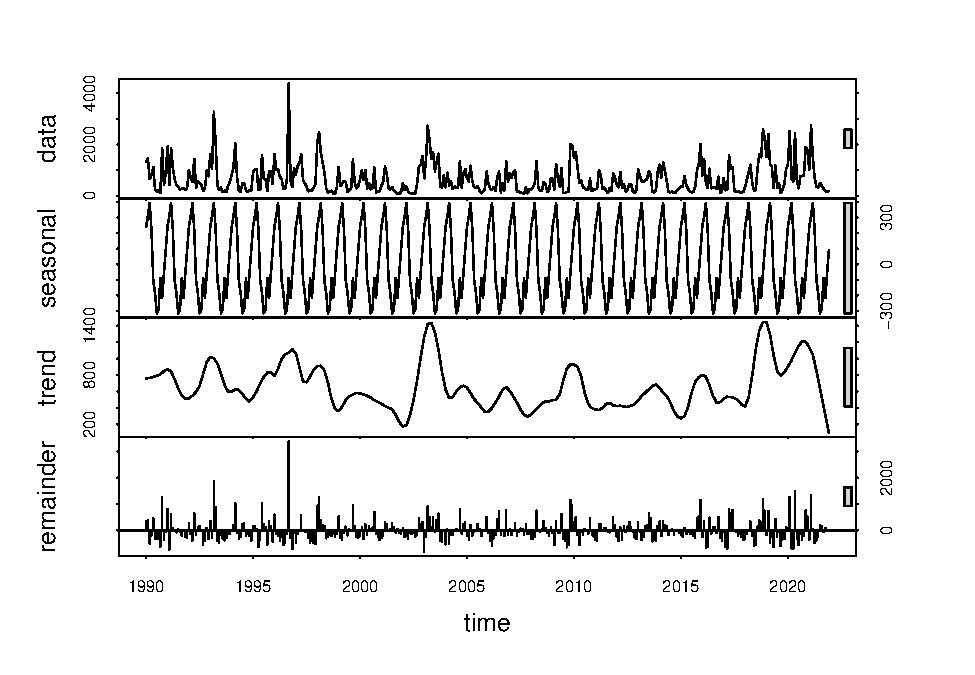
\includegraphics{Project_files/figure-latex/time-series analysis on Regular Water Resources-1.pdf}

\begin{Shaded}
\begin{Highlighting}[]
\NormalTok{CapeFearRiver\_trend }\OtherTok{\textless{}{-}} \FunctionTok{smk.test}\NormalTok{(CapeFearRiver\_timeseries)}
\NormalTok{CapeFearRiver\_trend}
\end{Highlighting}
\end{Shaded}

\begin{verbatim}
## 
##  Seasonal Mann-Kendall trend test (Hirsch-Slack test)
## 
## data:  CapeFearRiver_timeseries
## z = -0.98775, p-value = 0.3233
## alternative hypothesis: true S is not equal to 0
## sample estimates:
##     S  varS 
##  -212 45632
\end{verbatim}

\begin{Shaded}
\begin{Highlighting}[]
\FunctionTok{summary}\NormalTok{(CapeFearRiver\_trend)}
\end{Highlighting}
\end{Shaded}

\begin{verbatim}
## 
##  Seasonal Mann-Kendall trend test (Hirsch-Slack test)
## 
## data: CapeFearRiver_timeseries
## alternative hypothesis: two.sided
## 
## Statistics for individual seasons
## 
## H0
##                      S   varS    tau      z Pr(>|z|)  
## Season 1:   S = 0  -98 3802.7 -0.198 -1.573  0.11572  
## Season 2:   S = 0  -18 3802.7 -0.036 -0.276  0.78279  
## Season 3:   S = 0  -72 3802.7 -0.145 -1.151  0.24958  
## Season 4:   S = 0  -78 3802.7 -0.157 -1.249  0.21179  
## Season 5:   S = 0   32 3802.7  0.065  0.503  0.61517  
## Season 6:   S = 0   24 3802.7  0.048  0.373  0.70916  
## Season 7:   S = 0  -48 3802.7 -0.097 -0.762  0.44596  
## Season 8:   S = 0   24 3802.7  0.048  0.373  0.70916  
## Season 9:   S = 0   12 3802.7  0.024  0.178  0.85842  
## Season 10:   S = 0  -4 3802.7 -0.008 -0.049  0.96120  
## Season 11:   S = 0  -4 3802.7 -0.008 -0.049  0.96120  
## Season 12:   S = 0  18 3802.7  0.036  0.276  0.78279  
## ---
## Signif. codes:  0 '***' 0.001 '**' 0.01 '*' 0.05 '.' 0.1 ' ' 1
\end{verbatim}

\begin{Shaded}
\begin{Highlighting}[]
\CommentTok{\#p{-}value is 0.3233, so there is no trend present in Cape Fear River.}

\NormalTok{FlatRiver\_timeseries }\OtherTok{\textless{}{-}} \FunctionTok{ts}\NormalTok{(FlatRiverDischarge\_Monthly}\SpecialCharTok{$}\NormalTok{Mean\_Discharge\_Bymonth, }\AttributeTok{frequency =} \DecValTok{12}\NormalTok{,}
                           \AttributeTok{start =} \FunctionTok{c}\NormalTok{(}\DecValTok{1990}\NormalTok{, }\DecValTok{1}\NormalTok{, }\DecValTok{1}\NormalTok{), }\AttributeTok{end =} \FunctionTok{c}\NormalTok{(}\DecValTok{2021}\NormalTok{, }\DecValTok{12}\NormalTok{, }\DecValTok{1}\NormalTok{))}
\NormalTok{FlatRiver\_Decomposed }\OtherTok{\textless{}{-}} \FunctionTok{stl}\NormalTok{(FlatRiver\_timeseries, }\AttributeTok{s.window =} \StringTok{"periodic"}\NormalTok{)}
\FunctionTok{plot}\NormalTok{(FlatRiver\_Decomposed)}
\end{Highlighting}
\end{Shaded}

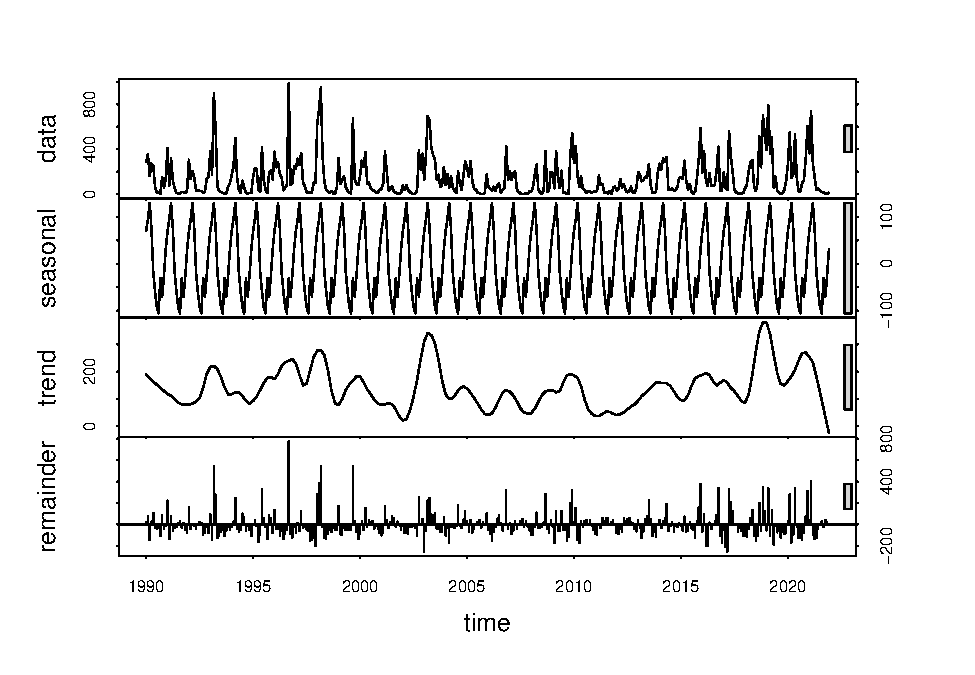
\includegraphics{Project_files/figure-latex/time-series analysis on Regular Water Resources-2.pdf}

\begin{Shaded}
\begin{Highlighting}[]
\NormalTok{FlatRiver\_trend }\OtherTok{\textless{}{-}} \FunctionTok{smk.test}\NormalTok{(FlatRiver\_timeseries)}
\NormalTok{FlatRiver\_trend}
\end{Highlighting}
\end{Shaded}

\begin{verbatim}
## 
##  Seasonal Mann-Kendall trend test (Hirsch-Slack test)
## 
## data:  FlatRiver_timeseries
## z = 0.84731, p-value = 0.3968
## alternative hypothesis: true S is not equal to 0
## sample estimates:
##     S  varS 
##   182 45632
\end{verbatim}

\begin{Shaded}
\begin{Highlighting}[]
\FunctionTok{summary}\NormalTok{(FlatRiver\_trend)}
\end{Highlighting}
\end{Shaded}

\begin{verbatim}
## 
##  Seasonal Mann-Kendall trend test (Hirsch-Slack test)
## 
## data: FlatRiver_timeseries
## alternative hypothesis: two.sided
## 
## Statistics for individual seasons
## 
## H0
##                      S   varS    tau      z Pr(>|z|)  
## Season 1:   S = 0  -76 3802.7 -0.153 -1.216 0.223896  
## Season 2:   S = 0    4 3802.7  0.008  0.049 0.961199  
## Season 3:   S = 0  -92 3802.7 -0.185 -1.476 0.140025  
## Season 4:   S = 0  -18 3802.7 -0.036 -0.276 0.782794  
## Season 5:   S = 0  108 3802.7  0.218  1.735 0.082712 .
## Season 6:   S = 0  110 3802.7  0.222  1.768 0.077129 .
## Season 7:   S = 0   38 3802.7  0.077  0.600 0.548500  
## Season 8:   S = 0   36 3802.7  0.073  0.568 0.570323  
## Season 9:   S = 0   58 3802.7  0.117  0.924 0.355310  
## Season 10:   S = 0 -18 3802.7 -0.036 -0.276 0.782794  
## Season 11:   S = 0   2 3802.7  0.004  0.016 0.987062  
## Season 12:   S = 0  30 3802.7  0.060  0.470 0.638157  
## ---
## Signif. codes:  0 '***' 0.001 '**' 0.01 '*' 0.05 '.' 0.1 ' ' 1
\end{verbatim}

\begin{Shaded}
\begin{Highlighting}[]
\CommentTok{\#p{-}value is 0.3968, so there is no trend present in Flat River.}

\NormalTok{LittleRiver\_timeseries }\OtherTok{\textless{}{-}} \FunctionTok{ts}\NormalTok{(LittleRiverDischarge\_Monthly}\SpecialCharTok{$}\NormalTok{Mean\_Discharge\_Bymonth, }\AttributeTok{frequency =} \DecValTok{12}\NormalTok{,}
                           \AttributeTok{start =} \FunctionTok{c}\NormalTok{(}\DecValTok{1990}\NormalTok{, }\DecValTok{1}\NormalTok{, }\DecValTok{1}\NormalTok{), }\AttributeTok{end =} \FunctionTok{c}\NormalTok{(}\DecValTok{2021}\NormalTok{, }\DecValTok{12}\NormalTok{, }\DecValTok{1}\NormalTok{))}
\NormalTok{LittleRiver\_Decomposed }\OtherTok{\textless{}{-}} \FunctionTok{stl}\NormalTok{(LittleRiver\_timeseries, }\AttributeTok{s.window =} \StringTok{"periodic"}\NormalTok{)}
\FunctionTok{plot}\NormalTok{(LittleRiver\_Decomposed)}
\end{Highlighting}
\end{Shaded}

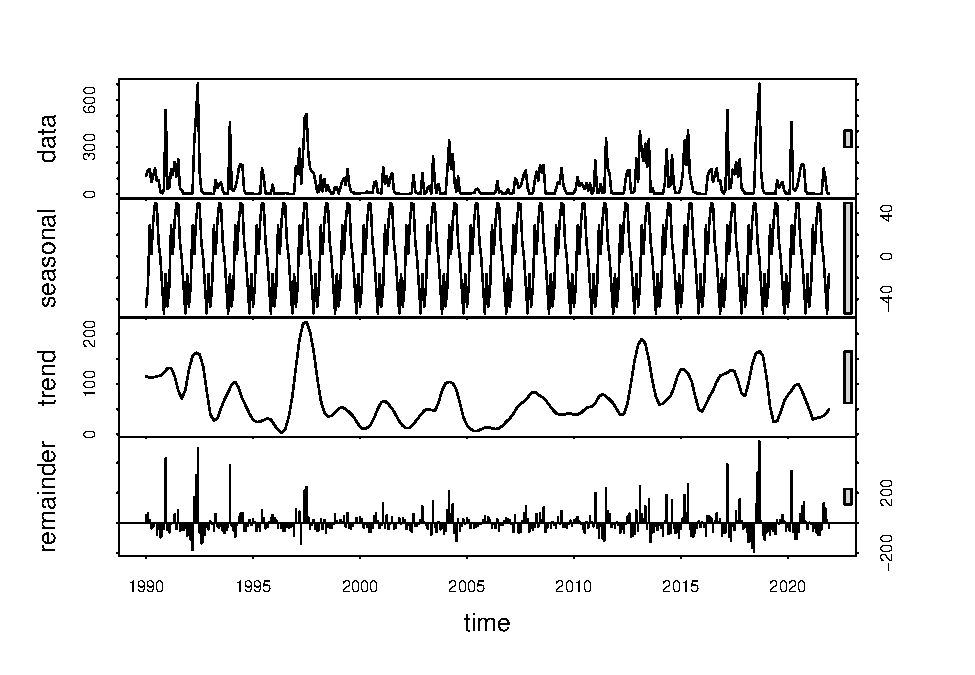
\includegraphics{Project_files/figure-latex/time-series analysis on Regular Water Resources-3.pdf}

\begin{Shaded}
\begin{Highlighting}[]
\NormalTok{LittleRiver\_trend }\OtherTok{\textless{}{-}} \FunctionTok{smk.test}\NormalTok{(LittleRiver\_timeseries)}
\NormalTok{LittleRiver\_trend}
\end{Highlighting}
\end{Shaded}

\begin{verbatim}
## 
##  Seasonal Mann-Kendall trend test (Hirsch-Slack test)
## 
## data:  LittleRiver_timeseries
## z = 0.82859, p-value = 0.4073
## alternative hypothesis: true S is not equal to 0
## sample estimates:
##     S  varS 
##   178 45632
\end{verbatim}

\begin{Shaded}
\begin{Highlighting}[]
\FunctionTok{summary}\NormalTok{(LittleRiver\_trend)}
\end{Highlighting}
\end{Shaded}

\begin{verbatim}
## 
##  Seasonal Mann-Kendall trend test (Hirsch-Slack test)
## 
## data: LittleRiver_timeseries
## alternative hypothesis: two.sided
## 
## Statistics for individual seasons
## 
## H0
##                       S   varS    tau      z  Pr(>|z|)   
## Season 1:   S = 0   -24 3802.7 -0.048 -0.373 0.7091645   
## Season 2:   S = 0   -60 3802.7 -0.121 -0.957 0.3386830   
## Season 3:   S = 0   -16 3802.7 -0.032 -0.243 0.8078142   
## Season 4:   S = 0   -72 3802.7 -0.145 -1.151 0.2495808   
## Season 5:   S = 0   -76 3802.7 -0.153 -1.216 0.2238958   
## Season 6:   S = 0  -120 3802.7 -0.242 -1.930 0.0536368  .
## Season 7:   S = 0   -18 3802.7 -0.036 -0.276 0.7827941   
## Season 8:   S = 0    94 3802.7  0.190  1.508 0.1315212   
## Season 9:   S = 0   202 3802.7  0.407  3.260 0.0011161 **
## Season 10:   S = 0  194 3802.7  0.391  3.130 0.0017494 **
## Season 11:   S = 0  126 3802.7  0.254  2.027 0.0426566  *
## Season 12:   S = 0  -52 3802.7 -0.105 -0.827 0.4082149   
## ---
## Signif. codes:  0 '***' 0.001 '**' 0.01 '*' 0.05 '.' 0.1 ' ' 1
\end{verbatim}

\begin{Shaded}
\begin{Highlighting}[]
\CommentTok{\#p{-}value is 0.4073, so there is no trend present in Little River.}
\end{Highlighting}
\end{Shaded}

\begin{Shaded}
\begin{Highlighting}[]
\CommentTok{\#Total Withdrawals}
\NormalTok{total\_withdrawal\_timeseries }\OtherTok{\textless{}{-}} \FunctionTok{ts}\NormalTok{(total\_withdrawal}\SpecialCharTok{$}\NormalTok{Avg\_Daily\_Use\_mgd, }\AttributeTok{frequency =} \DecValTok{12}\NormalTok{,}
                           \AttributeTok{start =} \FunctionTok{c}\NormalTok{(}\DecValTok{2018}\NormalTok{, }\DecValTok{1}\NormalTok{, }\DecValTok{1}\NormalTok{), }\AttributeTok{end =} \FunctionTok{c}\NormalTok{(}\DecValTok{2021}\NormalTok{, }\DecValTok{12}\NormalTok{, }\DecValTok{1}\NormalTok{))}
\NormalTok{total\_withdrawal\_Decomposed }\OtherTok{\textless{}{-}} \FunctionTok{stl}\NormalTok{(total\_withdrawal\_timeseries, }\AttributeTok{s.window =} \StringTok{"periodic"}\NormalTok{)}
\FunctionTok{plot}\NormalTok{(total\_withdrawal\_Decomposed)}
\end{Highlighting}
\end{Shaded}

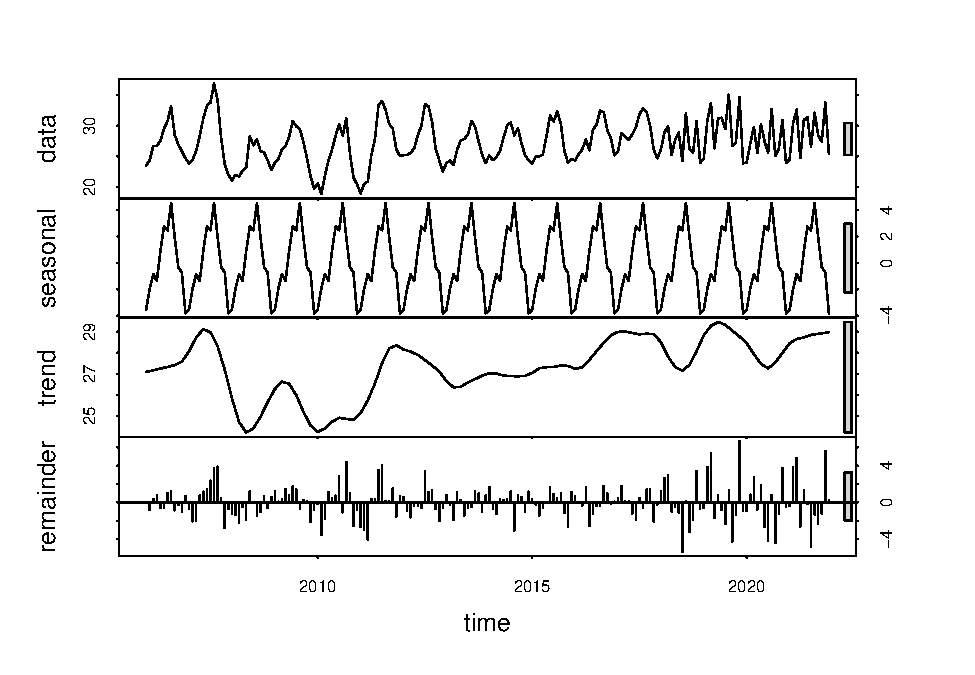
\includegraphics{Project_files/figure-latex/time-series analysis on withdrawals-1.pdf}

\begin{Shaded}
\begin{Highlighting}[]
\NormalTok{total\_withdrawal\_trend }\OtherTok{\textless{}{-}} \FunctionTok{smk.test}\NormalTok{(total\_withdrawal\_timeseries)}
\NormalTok{total\_withdrawal\_trend}
\end{Highlighting}
\end{Shaded}

\begin{verbatim}
## 
##  Seasonal Mann-Kendall trend test (Hirsch-Slack test)
## 
## data:  total_withdrawal_timeseries
## z = 0.88252, p-value = 0.3775
## alternative hypothesis: true S is not equal to 0
## sample estimates:
##    S varS 
##   10  104
\end{verbatim}

\begin{Shaded}
\begin{Highlighting}[]
\FunctionTok{summary}\NormalTok{(total\_withdrawal\_trend)}
\end{Highlighting}
\end{Shaded}

\begin{verbatim}
## 
##  Seasonal Mann-Kendall trend test (Hirsch-Slack test)
## 
## data: total_withdrawal_timeseries
## alternative hypothesis: two.sided
## 
## Statistics for individual seasons
## 
## H0
##                     S varS    tau      z Pr(>|z|)  
## Season 1:   S = 0  -4  8.7 -0.667 -1.019  0.30818  
## Season 2:   S = 0   0  8.7  0.000  0.000  1.00000  
## Season 3:   S = 0   0  8.7  0.000  0.000  1.00000  
## Season 4:   S = 0  -2  8.7 -0.333 -0.340  0.73410  
## Season 5:   S = 0   2  8.7  0.333  0.340  0.73410  
## Season 6:   S = 0   2  8.7  0.333  0.340  0.73410  
## Season 7:   S = 0   2  8.7  0.333  0.340  0.73410  
## Season 8:   S = 0   0  8.7  0.000  0.000  1.00000  
## Season 9:   S = 0   2  8.7  0.333  0.340  0.73410  
## Season 10:   S = 0  4  8.7  0.667  1.019  0.30818  
## Season 11:   S = 0  2  8.7  0.333  0.340  0.73410  
## Season 12:   S = 0  2  8.7  0.333  0.340  0.73410  
## ---
## Signif. codes:  0 '***' 0.001 '**' 0.01 '*' 0.05 '.' 0.1 ' ' 1
\end{verbatim}

\begin{Shaded}
\begin{Highlighting}[]
\CommentTok{\#p{-}value is 0.3775, so there is no trend present in Total Withdrawals.}
\end{Highlighting}
\end{Shaded}

\begin{Shaded}
\begin{Highlighting}[]
\NormalTok{DurhamGroundwater\_timeseries }\OtherTok{\textless{}{-}} \FunctionTok{ts}\NormalTok{(DurhamGroundwater}\SpecialCharTok{$}\NormalTok{Groundwater\_Table\_feet, }\AttributeTok{frequency =} \DecValTok{12}\NormalTok{,}
                           \AttributeTok{start =} \FunctionTok{c}\NormalTok{(}\DecValTok{2009}\NormalTok{, }\DecValTok{1}\NormalTok{, }\DecValTok{1}\NormalTok{), }\AttributeTok{end =} \FunctionTok{c}\NormalTok{(}\DecValTok{2021}\NormalTok{, }\DecValTok{12}\NormalTok{, }\DecValTok{1}\NormalTok{))}
\NormalTok{DurhamGroundwater\_Decomposed }\OtherTok{\textless{}{-}} \FunctionTok{stl}\NormalTok{(DurhamGroundwater\_timeseries, }\AttributeTok{s.window =} \StringTok{"periodic"}\NormalTok{)}
\FunctionTok{plot}\NormalTok{(DurhamGroundwater\_Decomposed)}
\end{Highlighting}
\end{Shaded}

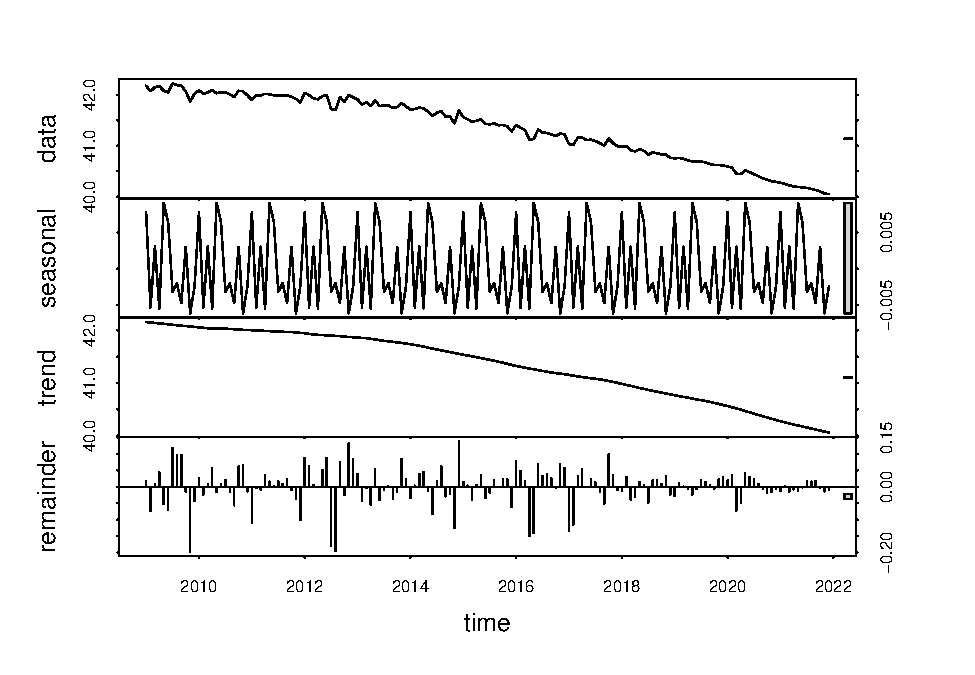
\includegraphics{Project_files/figure-latex/time-series analysis on groundwater-1.pdf}

\begin{Shaded}
\begin{Highlighting}[]
\NormalTok{DurhamGroundwater\_trend }\OtherTok{\textless{}{-}} \FunctionTok{smk.test}\NormalTok{(DurhamGroundwater\_timeseries)}
\NormalTok{DurhamGroundwater\_trend}
\end{Highlighting}
\end{Shaded}

\begin{verbatim}
## 
##  Seasonal Mann-Kendall trend test (Hirsch-Slack test)
## 
## data:  DurhamGroundwater_timeseries
## z = -15.964, p-value < 2.2e-16
## alternative hypothesis: true S is not equal to 0
## sample estimates:
##    S varS 
## -907 3221
\end{verbatim}

\begin{Shaded}
\begin{Highlighting}[]
\FunctionTok{summary}\NormalTok{(DurhamGroundwater\_trend)}
\end{Highlighting}
\end{Shaded}

\begin{verbatim}
## 
##  Seasonal Mann-Kendall trend test (Hirsch-Slack test)
## 
## data: DurhamGroundwater_timeseries
## alternative hypothesis: two.sided
## 
## Statistics for individual seasons
## 
## H0
##                      S  varS    tau      z   Pr(>|z|)    
## Season 1:   S = 0  -74 268.7 -0.949 -4.454 8.4423e-06 ***
## Season 2:   S = 0  -77 267.7 -0.994 -4.645 3.3954e-06 ***
## Season 3:   S = 0  -78 268.7 -1.000 -4.698 2.6313e-06 ***
## Season 4:   S = 0  -76 268.7 -0.974 -4.576 4.7471e-06 ***
## Season 5:   S = 0  -78 268.7 -1.000 -4.698 2.6313e-06 ***
## Season 6:   S = 0  -75 267.7 -0.968 -4.523 6.0945e-06 ***
## Season 7:   S = 0  -76 268.7 -0.974 -4.576 4.7471e-06 ***
## Season 8:   S = 0  -76 268.7 -0.974 -4.576 4.7471e-06 ***
## Season 9:   S = 0  -75 267.7 -0.968 -4.523 6.0945e-06 ***
## Season 10:   S = 0 -76 268.7 -0.974 -4.576 4.7471e-06 ***
## Season 11:   S = 0 -70 268.7 -0.897 -4.210 2.5581e-05 ***
## Season 12:   S = 0 -76 268.7 -0.974 -4.576 4.7471e-06 ***
## ---
## Signif. codes:  0 '***' 0.001 '**' 0.01 '*' 0.05 '.' 0.1 ' ' 1
\end{verbatim}

\begin{Shaded}
\begin{Highlighting}[]
\CommentTok{\#p{-}value is less than 0.05, so there is no trend present in Total Withdrawals.}
\end{Highlighting}
\end{Shaded}

\begin{Shaded}
\begin{Highlighting}[]
\NormalTok{DurhamPrecipitaion\_timeseries }\OtherTok{\textless{}{-}} \FunctionTok{ts}\NormalTok{(DurhamPrecipitaion}\SpecialCharTok{$}\NormalTok{Precipitaion\_inches, }\AttributeTok{frequency =} \DecValTok{12}\NormalTok{,}
                           \AttributeTok{start =} \FunctionTok{c}\NormalTok{(}\DecValTok{2009}\NormalTok{, }\DecValTok{1}\NormalTok{, }\DecValTok{1}\NormalTok{), }\AttributeTok{end =} \FunctionTok{c}\NormalTok{(}\DecValTok{2021}\NormalTok{, }\DecValTok{12}\NormalTok{, }\DecValTok{1}\NormalTok{))}
\NormalTok{DurhamPrecipitaion\_Decomposed }\OtherTok{\textless{}{-}} \FunctionTok{stl}\NormalTok{(DurhamPrecipitaion\_timeseries, }\AttributeTok{s.window =} \StringTok{"periodic"}\NormalTok{)}
\FunctionTok{plot}\NormalTok{(DurhamPrecipitaion\_Decomposed)}
\end{Highlighting}
\end{Shaded}

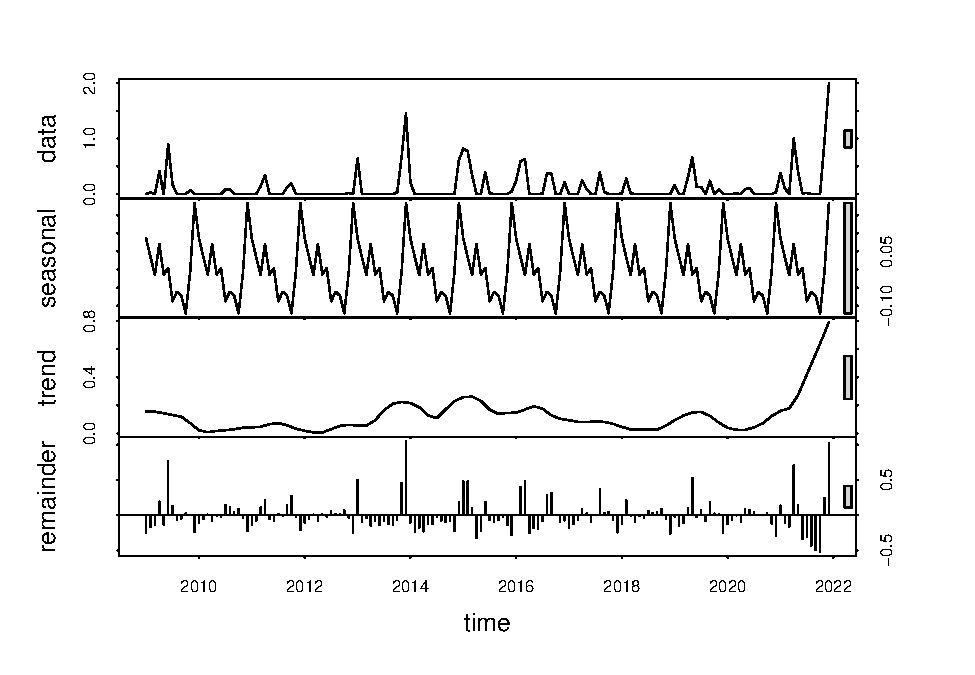
\includegraphics{Project_files/figure-latex/time-series analysis on precipitation-1.pdf}

\begin{Shaded}
\begin{Highlighting}[]
\NormalTok{DurhamPrecipitaion\_trend }\OtherTok{\textless{}{-}} \FunctionTok{smk.test}\NormalTok{(DurhamGroundwater\_timeseries)}
\NormalTok{DurhamPrecipitaion\_trend}
\end{Highlighting}
\end{Shaded}

\begin{verbatim}
## 
##  Seasonal Mann-Kendall trend test (Hirsch-Slack test)
## 
## data:  DurhamGroundwater_timeseries
## z = -15.964, p-value < 2.2e-16
## alternative hypothesis: true S is not equal to 0
## sample estimates:
##    S varS 
## -907 3221
\end{verbatim}

\begin{Shaded}
\begin{Highlighting}[]
\FunctionTok{summary}\NormalTok{(DurhamPrecipitaion\_trend)}
\end{Highlighting}
\end{Shaded}

\begin{verbatim}
## 
##  Seasonal Mann-Kendall trend test (Hirsch-Slack test)
## 
## data: DurhamGroundwater_timeseries
## alternative hypothesis: two.sided
## 
## Statistics for individual seasons
## 
## H0
##                      S  varS    tau      z   Pr(>|z|)    
## Season 1:   S = 0  -74 268.7 -0.949 -4.454 8.4423e-06 ***
## Season 2:   S = 0  -77 267.7 -0.994 -4.645 3.3954e-06 ***
## Season 3:   S = 0  -78 268.7 -1.000 -4.698 2.6313e-06 ***
## Season 4:   S = 0  -76 268.7 -0.974 -4.576 4.7471e-06 ***
## Season 5:   S = 0  -78 268.7 -1.000 -4.698 2.6313e-06 ***
## Season 6:   S = 0  -75 267.7 -0.968 -4.523 6.0945e-06 ***
## Season 7:   S = 0  -76 268.7 -0.974 -4.576 4.7471e-06 ***
## Season 8:   S = 0  -76 268.7 -0.974 -4.576 4.7471e-06 ***
## Season 9:   S = 0  -75 267.7 -0.968 -4.523 6.0945e-06 ***
## Season 10:   S = 0 -76 268.7 -0.974 -4.576 4.7471e-06 ***
## Season 11:   S = 0 -70 268.7 -0.897 -4.210 2.5581e-05 ***
## Season 12:   S = 0 -76 268.7 -0.974 -4.576 4.7471e-06 ***
## ---
## Signif. codes:  0 '***' 0.001 '**' 0.01 '*' 0.05 '.' 0.1 ' ' 1
\end{verbatim}

\hypertarget{question-1-insert-specific-question-here-and-add-additional-subsections-for-additional-questions-below-if-needed-is-there-a-relationship-between-surface-water-flow-and-groundwater-levels-in-durham-region}{%
\subsection{Question 1: \textless insert specific question here and add
additional subsections for additional questions below, if
needed\textgreater{} Is there a relationship between surface water flow
and groundwater levels in Durham
region?}\label{question-1-insert-specific-question-here-and-add-additional-subsections-for-additional-questions-below-if-needed-is-there-a-relationship-between-surface-water-flow-and-groundwater-levels-in-durham-region}}

\hypertarget{question-2-how-much-is-surface-water-affected-by-municipal-withdrawal-and-precipitation-recharge}{%
\subsection{Question 2: How much is surface water affected by municipal
withdrawal and precipitation
recharge?}\label{question-2-how-much-is-surface-water-affected-by-municipal-withdrawal-and-precipitation-recharge}}

\newpage

\hypertarget{summary-and-conclusions}{%
\section{Summary and Conclusions}\label{summary-and-conclusions}}

\newpage

\hypertarget{references}{%
\section{References}\label{references}}

\textless add references here if relevant, otherwise delete this
section\textgreater{}

\end{document}
